\documentclass{article}
\usepackage{tikz}
\title{How to Solve a Rubik's Cube Like a Computer}
\date{}
\author{}
\newcommand{\drawtop}[9]{
	\coordinate (v0) at (0, 1);
	\coordinate (v1) at (-0.288675, 0.833333);
	\coordinate (v2) at (0, 0.666667);
	\coordinate (v3) at (0.288675, 0.833333);
	\coordinate (v4) at (-0.577350, 0.666667);
	\coordinate (v5) at (-0.288675, 0.5);
	\coordinate (v6) at (0, 0.333333);
	\coordinate (v7) at (0.288675, 0.5);
	\coordinate (v8) at (0.577350, 0.666667);
	\coordinate (v9) at (-0.866025, 0.5);
	\coordinate (v10) at (-0.577350, 0.333333);
	\coordinate (v11) at (-0.288675, 0.166667);
	\coordinate (v12) at (0.288675, 0.166667);
	\coordinate (v13) at (0.577350, 0.333333);
	\coordinate (v14) at (0.866025, 0.5);
	\coordinate (v15) at (0, 0);

	\fill[color = #1] (v0) -- (v1) -- (v2) -- (v3);
	\fill[color = #2] (v1) -- (v4) -- (v5) -- (v2);
	\fill[color = #3] (v4) -- (v9) -- (v10) -- (v5);
	\fill[color = #4] (v10) -- (v11) -- (v6) -- (v5);
	\fill[color = #5] (v5) -- (v6) -- (v7) -- (v2);
	\fill[color = #6] (v2) -- (v7) -- (v8) -- (v3);
	\fill[color = #7] (v7) -- (v13) -- (v14) -- (v8);
	\fill[color = #8] (v6) -- (v12) -- (v13) -- (v7);
	\fill[color = #9] (v11) -- (v15) -- (v12) -- (v6);

	%Left-Up diagonal lines
	\draw[color = black] (v9) -- (v0);
	\draw[color = black] (v10) -- (v3);
	\draw[color = black] (v11) -- (v8);
	\draw[color = black] (v15) -- (v14);

	%Down-Right diagonal lines
	\draw[color = black] (v0) -- (v14);
}

\newcommand{\drawleft}[9]{
	\coordinate (v0) at (-0.866025, 0.5);
	\coordinate (v1) at (-0.577350, 0.333333);
	\coordinate (v2) at (-0.288675, 0.166667);
	\coordinate (v3) at (0, 0);
	\coordinate (v4) at (-0.866025, 0.166667);
	\coordinate (v5) at (-0.577350, 0.0);
	\coordinate (v6) at (-0.288675, -0.166667);
	\coordinate (v7) at (0, -0.333333);
	\coordinate (v8) at (-0.866025, -0.166667);
	\coordinate (v9) at (-0.577350, -0.333333);
	\coordinate (v10) at (-0.288675, -0.5);
	\coordinate (v11) at (0, -0.666667);
	\coordinate (v12) at (-0.866025, -0.5);
	\coordinate (v13) at (-0.577350, -0.666667);
	\coordinate (v14) at (-0.288675, -0.833333);
	\coordinate (v15) at (0, -1);

	\fill[color = #1] (v0) -- (v1) -- (v5) -- (v4);
	\fill[color = #2] (v1) -- (v2) -- (v6) -- (v5);
	\fill[color = #3] (v2) -- (v3) -- (v7) -- (v6);
	\fill[color = #4] (v4) -- (v5) -- (v9) -- (v8);
	\fill[color = #5] (v5) -- (v6) -- (v10) -- (v9);
	\fill[color = #6] (v6) -- (v7) -- (v11) -- (v10);
	\fill[color = #7] (v8) -- (v9) -- (v13) -- (v12);
	\fill[color = #8] (v9) -- (v10) -- (v14) -- (v13);
	\fill[color = #9] (v10) -- (v11) -- (v15) -- (v14);
}

\newcommand{\drawright}[9]{
	\coordinate (v0) at (0, 0);
	\coordinate (v1) at (0.288675, 0.166667);
	\coordinate (v2) at (0.577350, 0.333333);
	\coordinate (v3) at (0.866025, 0.5);
	\coordinate (v4) at (0, -0.333333);
	\coordinate (v5) at (0.288675, -0.166667);
	\coordinate (v6) at (0.577359, 0.0);
	\coordinate (v7) at (0.866025, 0.166667);
	\coordinate (v8) at (0, -0.666667);
	\coordinate (v9) at (0.288675, -0.5);
	\coordinate (v10) at (0.577359, -0.333333);
	\coordinate (v11) at (0.866025, -0.166667);
	\coordinate (v12) at (0, -1);
	\coordinate (v13) at (0.288675, -0.833333);
	\coordinate (v14) at (0.577359, -0.666667);
	\coordinate (v15) at (0.866025, -0.5);

	\fill[color = #1] (v0) -- (v1) -- (v5) -- (v4);
	\fill[color = #2] (v1) -- (v2) -- (v6) -- (v5);
	\fill[color = #3] (v2) -- (v3) -- (v7) -- (v6);
	\fill[color = #4] (v4) -- (v5) -- (v9) -- (v8);
	\fill[color = #5] (v5) -- (v6) -- (v10) -- (v9);
	\fill[color = #6] (v6) -- (v7) -- (v11) -- (v10);
	\fill[color = #7] (v8) -- (v9) -- (v13) -- (v12);
	\fill[color = #8] (v9) -- (v10) -- (v14) -- (v13);
	\fill[color = #9] (v10) -- (v11) -- (v15) -- (v14);
}


\newcommand{\step}{\vspace{0.25cm}\hrule\vspace{0.25cm}}

%%Template
\iffalse

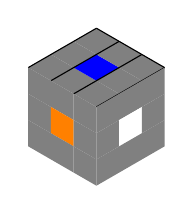
\begin{tikzpicture}[scale=1.0]
\drawtop{gray}{gray}{gray}{gray}{blue}{gray}{gray}{gray}{gray}
\drawleft{gray}{gray}{gray}{gray}{orange}{gray}{gray}{gray}{gray}
\drawright{gray}{gray}{gray}{gray}{white}{gray}{gray}{gray}{gray}
\end{tikzpicture}

\fi
%%

\begin{document}

%First step
Set \emph{solution number} to 0.

\step

%Orientation of the first corner
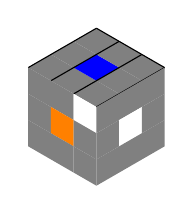
\begin{tikzpicture}[scale=1.0]
\drawtop{gray}{gray}{gray}{gray}{blue}{gray}{gray}{gray}{gray}
\drawleft{gray}{gray}{white}{gray}{orange}{gray}{gray}{gray}{gray}
\drawright{gray}{gray}{gray}{gray}{white}{gray}{gray}{gray}{gray}
\end{tikzpicture}
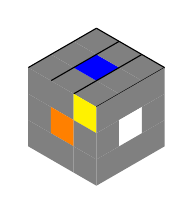
\begin{tikzpicture}[scale=1.0]
\drawtop{gray}{gray}{gray}{gray}{blue}{gray}{gray}{gray}{gray}
\drawleft{gray}{gray}{yellow}{gray}{orange}{gray}{gray}{gray}{gray}
\drawright{gray}{gray}{gray}{gray}{white}{gray}{gray}{gray}{gray}
\end{tikzpicture}

1. Add 495 to \emph{solution number}.

\step

%Orientation of the first corner
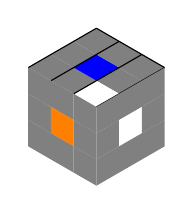
\begin{tikzpicture}[scale=1.0]
\drawtop{gray}{gray}{gray}{gray}{blue}{gray}{gray}{gray}{white}
\drawleft{gray}{gray}{gray}{gray}{orange}{gray}{gray}{gray}{gray}
\drawright{gray}{gray}{gray}{gray}{white}{gray}{gray}{gray}{gray}
\end{tikzpicture}
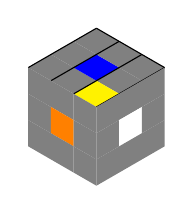
\begin{tikzpicture}[scale=1.0]
\drawtop{gray}{gray}{gray}{gray}{blue}{gray}{gray}{gray}{yellow}
\drawleft{gray}{gray}{gray}{gray}{orange}{gray}{gray}{gray}{gray}
\drawright{gray}{gray}{gray}{gray}{white}{gray}{gray}{gray}{gray}
\end{tikzpicture}

2. Add 990 to \emph{solution number}.

\step

%Orientation of the second corner
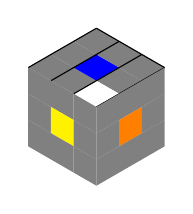
\begin{tikzpicture}[scale=1.0]
\drawtop{gray}{gray}{gray}{gray}{blue}{gray}{gray}{gray}{white}
\drawleft{gray}{gray}{gray}{gray}{yellow}{gray}{gray}{gray}{gray}
\drawright{gray}{gray}{gray}{gray}{orange}{gray}{gray}{gray}{gray}
\end{tikzpicture}
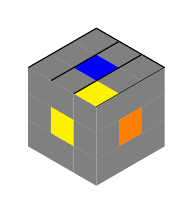
\begin{tikzpicture}[scale=1.0]
\drawtop{gray}{gray}{gray}{gray}{blue}{gray}{gray}{gray}{yellow}
\drawleft{gray}{gray}{gray}{gray}{yellow}{gray}{gray}{gray}{gray}
\drawright{gray}{gray}{gray}{gray}{orange}{gray}{gray}{gray}{gray}
\end{tikzpicture}

3. Add 1485 to \emph{solution number}.

\step

%Orientation of the second corner
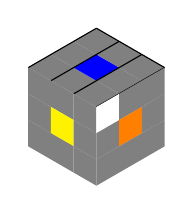
\begin{tikzpicture}[scale=1.0]
\drawtop{gray}{gray}{gray}{gray}{blue}{gray}{gray}{gray}{gray}
\drawleft{gray}{gray}{gray}{gray}{yellow}{gray}{gray}{gray}{gray}
\drawright{white}{gray}{gray}{gray}{orange}{gray}{gray}{gray}{gray}
\end{tikzpicture}
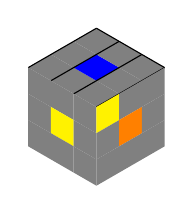
\begin{tikzpicture}[scale=1.0]
\drawtop{gray}{gray}{gray}{gray}{blue}{gray}{gray}{gray}{gray}
\drawleft{gray}{gray}{gray}{gray}{yellow}{gray}{gray}{gray}{gray}
\drawright{yellow}{gray}{gray}{gray}{orange}{gray}{gray}{gray}{gray}
\end{tikzpicture}

4. Add 2970 to \emph{solution number}.

\step

%Orientation of the third corner
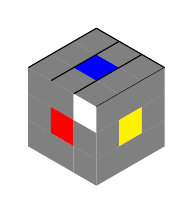
\begin{tikzpicture}[scale=1.0]
\drawtop{gray}{gray}{gray}{gray}{blue}{gray}{gray}{gray}{gray}
\drawleft{gray}{gray}{white}{gray}{red}{gray}{gray}{gray}{gray}
\drawright{gray}{gray}{gray}{gray}{yellow}{gray}{gray}{gray}{gray}
\end{tikzpicture}
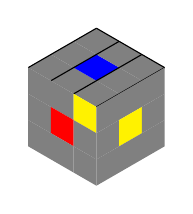
\begin{tikzpicture}[scale=1.0]
\drawtop{gray}{gray}{gray}{gray}{blue}{gray}{gray}{gray}{gray}
\drawleft{gray}{gray}{yellow}{gray}{red}{gray}{gray}{gray}{gray}
\drawright{gray}{gray}{gray}{gray}{yellow}{gray}{gray}{gray}{gray}
\end{tikzpicture}

5. Add 4455 to \emph{solution number}.

\step

%Orientation of the third corner
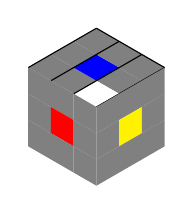
\begin{tikzpicture}[scale=1.0]
\drawtop{gray}{gray}{gray}{gray}{blue}{gray}{gray}{gray}{white}
\drawleft{gray}{gray}{gray}{gray}{red}{gray}{gray}{gray}{gray}
\drawright{gray}{gray}{gray}{gray}{yellow}{gray}{gray}{gray}{gray}
\end{tikzpicture}
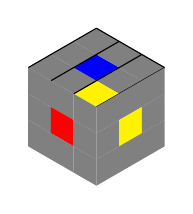
\begin{tikzpicture}[scale=1.0]
\drawtop{gray}{gray}{gray}{gray}{blue}{gray}{gray}{gray}{yellow}
\drawleft{gray}{gray}{gray}{gray}{red}{gray}{gray}{gray}{gray}
\drawright{gray}{gray}{gray}{gray}{yellow}{gray}{gray}{gray}{gray}
\end{tikzpicture}

6. Add 8910 to \emph{solution number}.

\step

%Orientation of the fourth corner
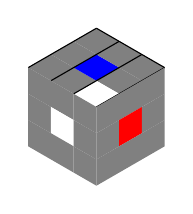
\begin{tikzpicture}[scale=1.0]
\drawtop{gray}{gray}{gray}{gray}{blue}{gray}{gray}{gray}{white}
\drawleft{gray}{gray}{gray}{gray}{white}{gray}{gray}{gray}{gray}
\drawright{gray}{gray}{gray}{gray}{red}{gray}{gray}{gray}{gray}
\end{tikzpicture}
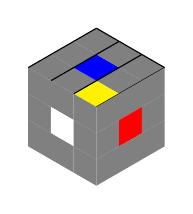
\begin{tikzpicture}[scale=1.0]
\drawtop{gray}{gray}{gray}{gray}{blue}{gray}{gray}{gray}{yellow}
\drawleft{gray}{gray}{gray}{gray}{white}{gray}{gray}{gray}{gray}
\drawright{gray}{gray}{gray}{gray}{red}{gray}{gray}{gray}{gray}
\end{tikzpicture}

7. Add 13365 to \emph{solution number}.

\step

%Orientation of the fourth corner
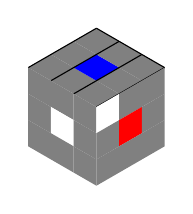
\begin{tikzpicture}[scale=1.0]
\drawtop{gray}{gray}{gray}{gray}{blue}{gray}{gray}{gray}{gray}
\drawleft{gray}{gray}{gray}{gray}{white}{gray}{gray}{gray}{gray}
\drawright{white}{gray}{gray}{gray}{red}{gray}{gray}{gray}{gray}
\end{tikzpicture}
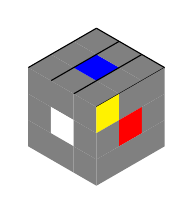
\begin{tikzpicture}[scale=1.0]
\drawtop{gray}{gray}{gray}{gray}{blue}{gray}{gray}{gray}{gray}
\drawleft{gray}{gray}{gray}{gray}{white}{gray}{gray}{gray}{gray}
\drawright{yellow}{gray}{gray}{gray}{red}{gray}{gray}{gray}{gray}
\end{tikzpicture}

8. Add 26730 to \emph{solution number}.

\step

%Orientation of the fifth corner
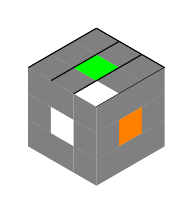
\begin{tikzpicture}[scale=1.0]
\drawtop{gray}{gray}{gray}{gray}{green}{gray}{gray}{gray}{white}
\drawleft{gray}{gray}{gray}{gray}{white}{gray}{gray}{gray}{gray}
\drawright{gray}{gray}{gray}{gray}{orange}{gray}{gray}{gray}{gray}
\end{tikzpicture}
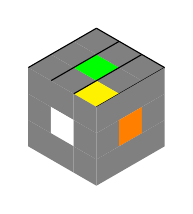
\begin{tikzpicture}[scale=1.0]
\drawtop{gray}{gray}{gray}{gray}{green}{gray}{gray}{gray}{yellow}
\drawleft{gray}{gray}{gray}{gray}{white}{gray}{gray}{gray}{gray}
\drawright{gray}{gray}{gray}{gray}{orange}{gray}{gray}{gray}{gray}
\end{tikzpicture}

9. Add 40095 to \emph{solution number}.

\step

%Orientation of the fifth corner
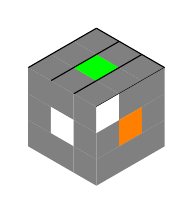
\begin{tikzpicture}[scale=1.0]
\drawtop{gray}{gray}{gray}{gray}{green}{gray}{gray}{gray}{gray}
\drawleft{gray}{gray}{gray}{gray}{white}{gray}{gray}{gray}{gray}
\drawright{white}{gray}{gray}{gray}{orange}{gray}{gray}{gray}{gray}
\end{tikzpicture}
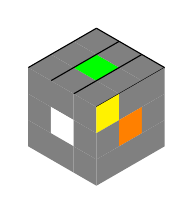
\begin{tikzpicture}[scale=1.0]
\drawtop{gray}{gray}{gray}{gray}{green}{gray}{gray}{gray}{gray}
\drawleft{gray}{gray}{gray}{gray}{white}{gray}{gray}{gray}{gray}
\drawright{yellow}{gray}{gray}{gray}{orange}{gray}{gray}{gray}{gray}
\end{tikzpicture}

10. Add 80190 to \emph{solution number}.

\step

%Orientation of the sixth corner
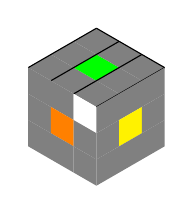
\begin{tikzpicture}[scale=1.0]
\drawtop{gray}{gray}{gray}{gray}{green}{gray}{gray}{gray}{gray}
\drawleft{gray}{gray}{white}{gray}{orange}{gray}{gray}{gray}{gray}
\drawright{gray}{gray}{gray}{gray}{yellow}{gray}{gray}{gray}{gray}
\end{tikzpicture}
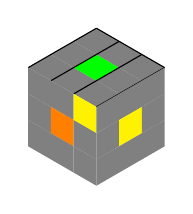
\begin{tikzpicture}[scale=1.0]
\drawtop{gray}{gray}{gray}{gray}{green}{gray}{gray}{gray}{gray}
\drawleft{gray}{gray}{yellow}{gray}{orange}{gray}{gray}{gray}{gray}
\drawright{gray}{gray}{gray}{gray}{yellow}{gray}{gray}{gray}{gray}
\end{tikzpicture}

11. Add 120285 to \emph{solution number}.

\step

%Orientation of the sixth corner
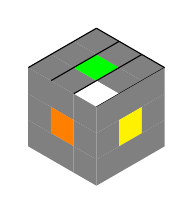
\begin{tikzpicture}[scale=1.0]
\drawtop{gray}{gray}{gray}{gray}{green}{gray}{gray}{gray}{white}
\drawleft{gray}{gray}{gray}{gray}{orange}{gray}{gray}{gray}{gray}
\drawright{gray}{gray}{gray}{gray}{yellow}{gray}{gray}{gray}{gray}
\end{tikzpicture}
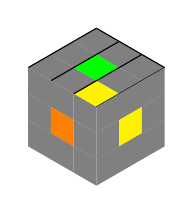
\begin{tikzpicture}[scale=1.0]
\drawtop{gray}{gray}{gray}{gray}{green}{gray}{gray}{gray}{yellow}
\drawleft{gray}{gray}{gray}{gray}{orange}{gray}{gray}{gray}{gray}
\drawright{gray}{gray}{gray}{gray}{yellow}{gray}{gray}{gray}{gray}
\end{tikzpicture}

12. Add 240570 to \emph{solution number}.

\step

%Orientation of the seventh corner
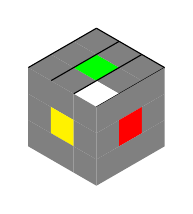
\begin{tikzpicture}[scale=1.0]
\drawtop{gray}{gray}{gray}{gray}{green}{gray}{gray}{gray}{white}
\drawleft{gray}{gray}{gray}{gray}{yellow}{gray}{gray}{gray}{gray}
\drawright{gray}{gray}{gray}{gray}{red}{gray}{gray}{gray}{gray}
\end{tikzpicture}
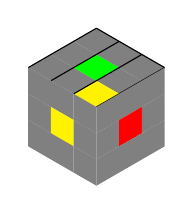
\begin{tikzpicture}[scale=1.0]
\drawtop{gray}{gray}{gray}{gray}{green}{gray}{gray}{gray}{yellow}
\drawleft{gray}{gray}{gray}{gray}{yellow}{gray}{gray}{gray}{gray}
\drawright{gray}{gray}{gray}{gray}{red}{gray}{gray}{gray}{gray}
\end{tikzpicture}

13. Add 360855 to \emph{solution number}.

\step

%Orientation of the seventh corner
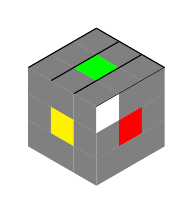
\begin{tikzpicture}[scale=1.0]
\drawtop{gray}{gray}{gray}{gray}{green}{gray}{gray}{gray}{gray}
\drawleft{gray}{gray}{gray}{gray}{yellow}{gray}{gray}{gray}{gray}
\drawright{white}{gray}{gray}{gray}{red}{gray}{gray}{gray}{gray}
\end{tikzpicture}
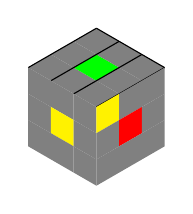
\begin{tikzpicture}[scale=1.0]
\drawtop{gray}{gray}{gray}{gray}{green}{gray}{gray}{gray}{gray}
\drawleft{gray}{gray}{gray}{gray}{yellow}{gray}{gray}{gray}{gray}
\drawright{yellow}{gray}{gray}{gray}{red}{gray}{gray}{gray}{gray}
\end{tikzpicture}

14. Add 721710 to \emph{solution number}.

\step
%Now I have to implement the combination of the middle edges
%I'm not quite sure how I'm going to do this

%12 choose 4 - edge position 0
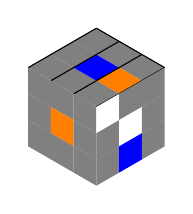
\begin{tikzpicture}[scale=1.0]
\drawtop{gray}{gray}{gray}{gray}{blue}{gray}{gray}{orange}{gray}
\drawleft{gray}{gray}{gray}{gray}{orange}{gray}{gray}{gray}{gray}
\drawright{white}{gray}{gray}{gray}{white}{gray}{gray}{blue}{gray}
\end{tikzpicture}

\end{document}
